\section{Repetition-Aware Mixture Scaling Law}
\label{sec:scaling_law}

The goal of this section is to quantify the empirical findings of Section~\ref{sec:results}.
We use scaling laws~\citep{kaplan2020scaling}, which, in their original forms, are simple power laws that allow to predict the train loss of a model from its number of parameters $N$ and total number of tokens it has been trained on $D_\text{total}$.
In our setup, both the target data size $D_\text{target}$ and the target weight $h$ influence the loss on the target domain. 
Our objective is to obtain a simple and predictive formula for $L_\text{target}(N, D_\text{total},  D_\text{target}, h)$.
We focus on the practically relevant regime where the target data is fully consumed at least once, i.e. $r = h \cdot D_\text{total} / D_\text{target} \ge 1$.
When $r < 1$, target tokens are never repeated and mixing reduces to standard mixture selection, as explored, e.g., in \citep{shukor2025scalinglawsoptimaldata}. In the following, we write scaling laws learned parameters in \pp{blue}.

\paragraph{Effective data} 
The core building block of our law is the \emph{effective data} $D_{\mathrm{eff}}$, which accounts for the diminishing value of repeated tokens.
Following \citet{muennighoff2023scaling}, we define the effective contribution of the \emph{target} domain as
\begin{equation}\label{eq:rho}
  D_T = D_\text{target}\bigl(1 + \rho(r)\bigr)\,,
  \qquad \text{with} \quad
  \rho(r) = \pp{r_1}\!\left(1 - e^{-(r-1)/\pp{r_1}}\right),
\end{equation}
where $\pp{r_1}$ is a parameter that controls the effect repeated data.
For small $r \ll \pp{r_1} + 1$, we have $\rho(r) \approx r - 1$ so that $D_T \approx r \cdot D_\text{target}$: each pass counts fully.
For large $r$, $D_T$ saturates at $(1 + \pp{r_1})\,D_\text{target}$, reflecting the diminishing value of further repetitions.
The total effective data is then
\begin{equation}\label{eq:deff}
  D_{\mathrm{eff}} = (1-h)\,D_\text{total} + \pp{\tau}\,D_T\,,
\end{equation}
where the  $(1-h)\,D_\text{total}$ term corresponds to the number of tokens seen from the generic dataset and $\pp{\tau}$ controls the relative value of target-domain tokens compared to generic-domain tokens.
This formulation directly encodes two observations from Section~\ref{sec:results}. The saturation of $\rho(r)$ at $\pp{r_1}$ is the quantitative form of the diminishing value of repeated target tokens: for $r \gg \pp{r_1}$, further passes add essentially nothing to $D_\mathrm{eff}$. Conversely, the unsaturated $(1-h)\,D_\text{total}$ term formalises why mixture training tolerates far more repetition than single-source training (Figure~\ref{fig:optimal_r}): generic tokens never saturate, so they keep $D_\mathrm{eff}$ growing even when the target contribution has plateaued.

\paragraph{Scaling law formulas}
We propose two loss formulas, for fixed and variable model size:
\begin{equation}\label{eq:lsize}
  L_{\mathrm{fix}} = \pp{E} + \frac{\pp{A}}{D_{\mathrm{eff}}^{\,\pp{\alpha}}} + \pp{\gamma}\,h\,,
  \qquad
  L_{\mathrm{size}} = \pp{E} + \frac{\pp{C}}{N^{\pp{\beta}}} + \frac{\pp{B} \, N^{\pp{\delta}}}{D_{\mathrm{eff}}^{\,\pp{\alpha}}} + \pp{\gamma}\,h\,.
\end{equation}
In $L_\mathrm{fix}$, the irreducible loss $\pp{E}$ is a constant baseline; the data term $\pp{A}/D_{\mathrm{eff}}^{\,\pp{\alpha}}$ is a Chinchilla-style power-law relating loss to effective data; and the weight penalty $\pp{\gamma}\,h$ is a linear cost on the target weight.
$L_\mathrm{size}$ additionally includes a Chinchilla-style capacity term $\pp{C}/N^{\pp{\beta}}$ and a data-size coupling $N^{\pp{\delta}}$ ($\pp{\delta} > 0$)~\citep{hoffmann2022training}: the capacity term captures the intrinsic capability gain from scale, while the coupling means that for the same $D_\mathrm{eff}$, the data-limited loss component is amplified at larger~$N$, encoding the fact that larger models yield better losses but overfit faster (Figure~\ref{fig:cross_model_fixed_h}).
At fixed $N$, $L_\mathrm{size}$ reduces exactly to $L_\mathrm{fix}$ with $\pp{A} = \pp{B}\,N^{\pp{\delta}}$ and $E_{\mathrm{fix}} = \pp{E} + \pp{C}/N^{\pp{\beta}}$, ensuring consistency.
$L_\mathrm{fix}$ has six fitted parameters ($\pp{E}$, $\pp{A}$, $\pp{\alpha}$, $\pp{r_1}$, $\pp{\tau}$, $\pp{\gamma}$); $L_\mathrm{size}$ has nine ($\pp{E}$, $\pp{C}$, $\pp{\beta}$, $\pp{B}$, $\pp{\delta}$, $\pp{\alpha}$, $\pp{r_1}$, $\pp{\tau}$, $\pp{\gamma}$).


\paragraph{Fitting}
Given a collection of training runs indexed by $i$, each characterised by a total token budget $D_{\text{total},i}$, a target weight $h_i$, an available target dataset $D_{\text{target},i}$, and optionally a model size $N_i$, we observe the resulting loss on the target domain $\ell_i$.
The parameters $\theta$ of the scaling law are estimated by minimising the reweighted Huber loss
\begin{equation}\label{eq:fit}
  \hat\theta = \arg\min_\theta \sum_i \omega_i \cdot \mathcal{H}\!\bigl(\ell_i - L_\theta(D_{\text{total},i},\, h_i,\, D_{\text{target},i},\, N_i)\bigr)\,,
\end{equation}
where $\mathcal{H}$ is the Huber loss and the weights $\omega_i = \max(r_i \cdot h_i,\, \epsilon)$ with $\epsilon=0.01$ emphasise the high-repetition, high-fraction regime: $h$ alone would under-weight high-repetition runs at moderate fractions, while $r$ alone would under-weight high-fraction runs with large datasets (where $r$ is low).
The qualitative ranking of methods is unchanged under alternative weights; see Appendix~\ref{app:weighting}.
Following~\citet{shukor2025scalinglawsoptimaldata}, we minimise~\ref{eq:fit} using basin-hopping optimisation with 100 random restarts to avoid poor local minima in the non-convex loss landscape.


\section{Scaling Law Results}
\label{sec:scaling_results}
We evaluate the scaling law on experimental setups described in Section~\ref{sec:datasets}.
For each setup, $L_\mathrm{fix}$ is fitted independently per model size, and $L_\mathrm{size}$ is fitted jointly across all model sizes.
To test extrapolation for $L_\mathrm{fix}$, we fit on the first 50\% of training steps and test on second half. For $L_\mathrm{size}$, we fit on all but the largest model scale, and test on the held-out largest model scale.

\begin{table}[t]
\centering
\caption{Test weighted $R^2$. \textbf{Left:} fixed-size formulas, fitted independently per model size. \textbf{Right:} multi-size formulas, fitted on smaller model sizes and evaluated on the held-out largest model.}
\label{tab:scaling_r2}\label{tab:scaling_r2_size}
\setlength{\tabcolsep}{3pt}
\begin{tabular}{lcccc|lcc}
\toprule
& German & Maths & Quality & Wiki/peS2o & & German & Maths \\
\midrule
$L_\mathrm{fix}$ & \textbf{0.95} & \textbf{0.88} & \textbf{0.71} & \textbf{0.80} & $L_\mathrm{size}$ & \textbf{0.65} & \textbf{0.73} \\
Repetition-agnostic & 0.78 & 0.78 & 0.14 & 0.72 & Repetition-agnostic+$N$ & 0.59 & 0.71 \\
Utility decay & 0.72 & 0.55 & $-$0.64 & 0.79 & Utility decay+$N$ & 0.56 & 0.69 \\
Domain-agnostic & $-$40.7 & $-$0.49 & $-$2.19 & $-$1.16 & Domain-agnostic+$N$ & $-$0.23 & $-$0.77 \\
\bottomrule
\vspace{-15pt}
\end{tabular}
\end{table}


\paragraph{Baselines}
We compare against three other scaling laws formulas inspired by the literature.
\emph{Repetitions-agnostic}~\citep{shukor2025scalinglawsoptimaldata} replaces $D_\mathrm{eff}$ with $(1-h)\,D_\text{total} + \pp{\tau}\,h\,D_\text{total}$, treating repeated tokens as unique.
\emph{Domain-agnostic}~\citep{muennighoff2023scaling} uses a single saturating function of total tokens without distinguishing domains.
\emph{Utility decay}~\citep{goyal2024scaling} models repetition through a decaying exponent on the data term.
The formulas are detailed in  Appendix~\ref{app:details}.

\paragraph{Optimal mixture prediction}
\begin{wrapfigure}{r}{0.38\textwidth}
\centering
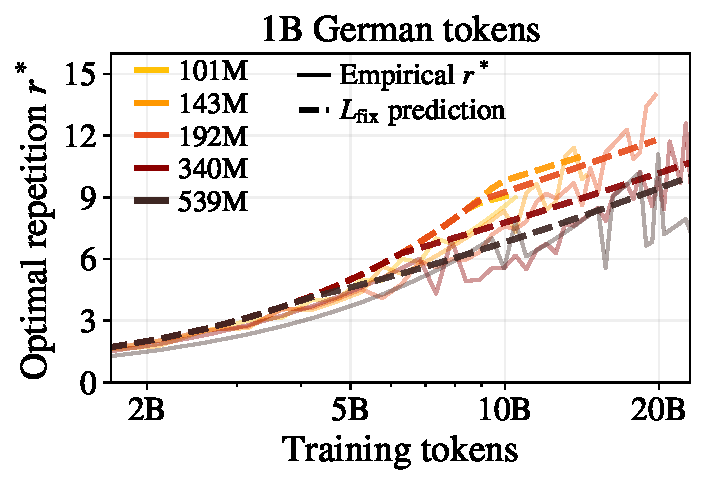
\includegraphics[width=0.37\textwidth]{figures/plot_predicted_vs_actual_r.pdf}
\caption{Predicted vs.\ empirical optimal repetition $r^*$ for the  German target dataset of 1B tokens. Solid: empirical optimum; dashed: $L_\mathrm{fix}$ prediction.}
\label{fig:predicted_vs_actual_r}
\vspace{-25pt}
\end{wrapfigure}

\paragraph{Loss prediction}
Table~\ref{tab:scaling_r2} reports the weighted coefficient of determination ($wR^2$) on the held-out test split (train $wR^2$ in Appendix~\ref{app:extended_scaling}), where each observation is weighted by $\max(r \cdot h,\, \epsilon)$ to emphasise the high-repetition regime.
$L_\mathrm{fix}$ consistently achieves the best test $wR^2$, extrapolating beyond the fitting range.
\emph{Repetitions-agnostic} fits the training range reasonably but fails to extrapolate to high repetitions. \emph{Domain agnostic} fails completely: treating all tokens as interchangeable does not capture the loss dynamics.
\emph{Utility decay} performs honorably on several datasets.

\begin{wrapfigure}{r}{0.35\textwidth}
\vspace{-10pt}
\centering
\footnotesize
\setlength{\tabcolsep}{4pt}
\begin{tabular}{lccc}
\toprule
& Median & Mean & p90 \\
\midrule
$L_\mathrm{fix}$ & \textbf{26} & \textbf{34} & \textbf{76} \\
Rep-agn. & 88 & 73 & 99 \\
Util. dec. & 31 & 41 & 95 \\
Dom.-agn. & 47 & 59 & 98 \\
\bottomrule
\end{tabular}
\captionof{table}{Fraction of training tokens wasted by following each formula's predicted optimal mixture instead of the oracle.}
\label{tab:scaling_weight}
\vspace{-10pt}
\end{wrapfigure}
The primary use of the scaling law is to predict the optimal target weight~$h^*$ for a given total token budget $D_\text{total}$ and available target domain dataset $D_\text{target}$.
Once the scaling law parameters are estimated, we can simply solve
\begin{equation}\label{eq:hstar}
  h^* = \arg\min_{h \in [0,1]} L_\mathrm{fix}(D_\text{total},\, h,\, D_\text{target})
\end{equation}
by grid search over~$h$. Figure~\ref{fig:predicted_vs_actual_r} shows an example of empirical vs. estimated optimal repetition.

To quantify the practical cost of suboptimal mixture predictions, we measure the fraction of training tokens \emph{wasted} by following each formula's recommendation instead of the oracle (Table~\ref{tab:scaling_weight}).
At a given budget $D_\text{total}$, the formula recommends a fraction~$h^*_\text{pred}$; we interpolate the empirical loss at that fraction and find the budget $D'$ at which the run using the empirically best fraction at each step first reached the same loss.
The wasted fraction $(D_\text{total} - D') / D_\text{total}$ directly measures how much compute could have been saved with perfect knowledge of the optimal mixture.
Detailed results are in Appendix~\ref{app:extended_scaling}.
